\begin{frame}
    \frametitle{Test de Kruskal-Wallis}
    % import image with a description
    La distribución de las notas de los estudiantes de la academia Trilce
    de acuerdo a sede es la siguiente: 
    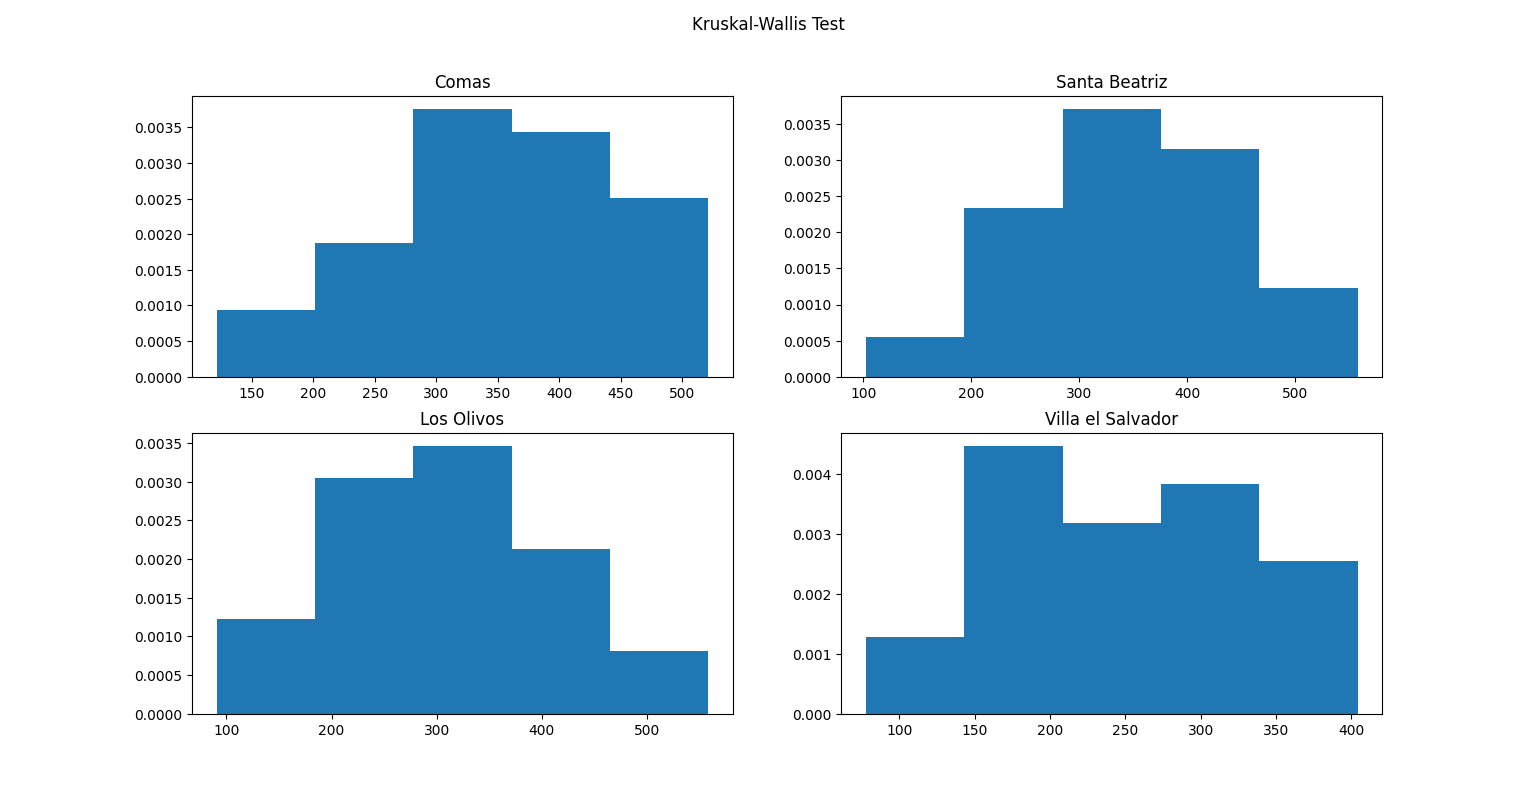
\includegraphics[width=1\textwidth]{cap/images/kruskal.png}
\end{frame}

\begin{frame}
    \frametitle{Test de Kruskal-Wallis}
    % import image with a description
    Con un gráfico de cajas se puede observar que la distribución de 
    Villa el Salvador tiene una mediana muestral que es distinta a las demás. 
    \centering
    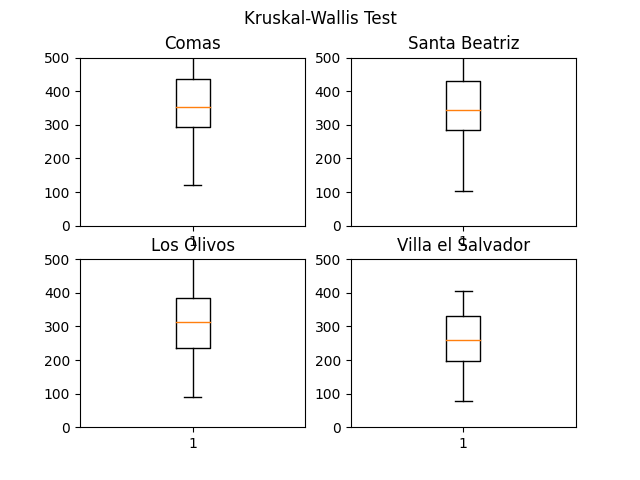
\includegraphics[width=0.8\textwidth]{cap/images/kruskal_boxplot.png}
\end{frame}

\begin{frame}
    \frametitle{Test de Kruskal-Wallis}
    % import image with a description
    \begin{itemize}
        \item Sea la hipótesis nula $H_0$ es que las distribuciones de las notas de los estudiantes de la academia Trilce de acuerdo a sede son iguales.
        \item La hipótesis alternativa $H_1$ es que al menos una de las distribuciones es distinta.
    \end{itemize}
    \begin{itemize}
        \item La prueba de Kruskal-Wallis arroja los siguientes resulados:
        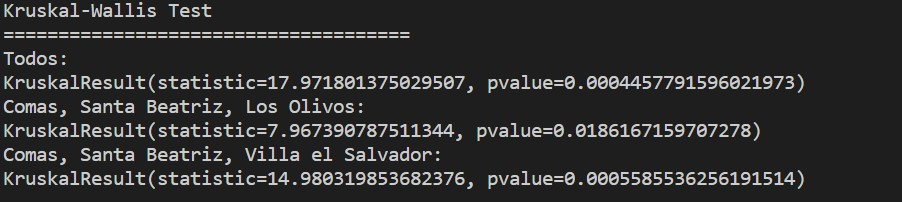
\includegraphics[width=0.8\textwidth]{cap/images/resultados_kruskal.jpg}
        \item Se rechaza $H_0$ y se concluye que al menos alguna distribución de notas de los estudiantes de la academia Trilce de acuerdo a sede difiere con un nivel de significancia del 5\%
    \end{itemize}
\end{frame}

\begin{frame}
    \frametitle{Test de Kruskal-Wallis}
    % import image with a description
    Al comparar las cuatro distribuciones el p-value es 0.000445. 
    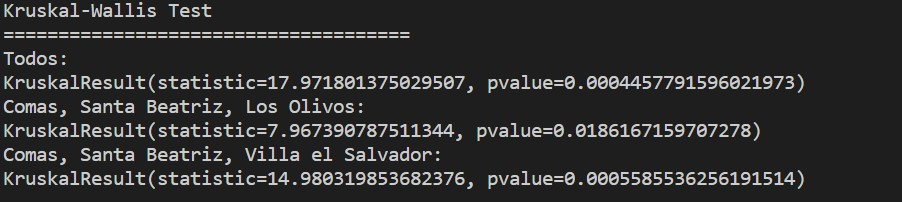
\includegraphics[width=0.8\textwidth]{cap/images/resultados_kruskal.jpg}
    
    Sin embargo, un detalle que resalta es que al excluir la distribución de Villa el Salvador, el p-value es 0.0186.
    Este valor sería significativo para un nivel de confianza del 1\% y señala una posible 
    diferencia que consideramos que es susceptible de futura investigación.
    
\end{frame}